\documentclass[aspectratio=169]{beamer}

\usetheme{Madrid}
\usecolortheme{default}

\usepackage[russian]{babel}
\usepackage{minted}
\usepackage{hyperref}
\usepackage{graphicx}

\title{Разработка клиентской части онлайн-форума SemiColon} 
\author{Выполнил: Кормышев Егор ИСиП-301}


\begin{document}

\frame{\titlepage}

% Frame 2: http requiests definitions 

\begin{frame}
  \frametitle{Онлайн форум SemiColon}
  
  \begin{center}
    \huge{Актуальность}
  \end{center}
  
  \begin{center}
    В современном мире информационных технологий, программирование становится все более популярной профессией. Многие люди, особенно те, кто переходит из других профессий, ищутся возможностей для обучения и развития в этой области. Поэтому создание онлайн-форума для программистов может стать полезным инструментом для обмена опытом, знаниями и решения проблем.

  \end{center}

\end{frame}

\begin{frame}
  \frametitle{Онлайн форум SemiColon}

  
  \begin{center}
    \huge{Цели и Задачи}
  \end{center}
  
  \large{Цель:}
  Целью курсового проекта является разработать дизайн \\ и пользовательский интерфейс для онлайн-форума. \\
  \bigskip

  \large{Задачи:}    
  \begin{itemize}
  \item Провести анализ предметной области
  \item Разработать информационную структуру приложения
  \item Разработать дизайн макета приложения
  \item Реализовать макет приложения
  \end{itemize}
  
\end{frame}


\begin{frame}
  \frametitle{Онлайн форум SemiColon}
  
  \begin{center}
    \huge{Предметная область}
  \end{center}
  
  \begin{center}
    В результате анализа предметной области были выделен \\
    основной бизнесс-процесс - \large{\textbf{Обмен информацией}}     
  \end{center}

  \begin{center}
    \begin{figure}
      \centering
      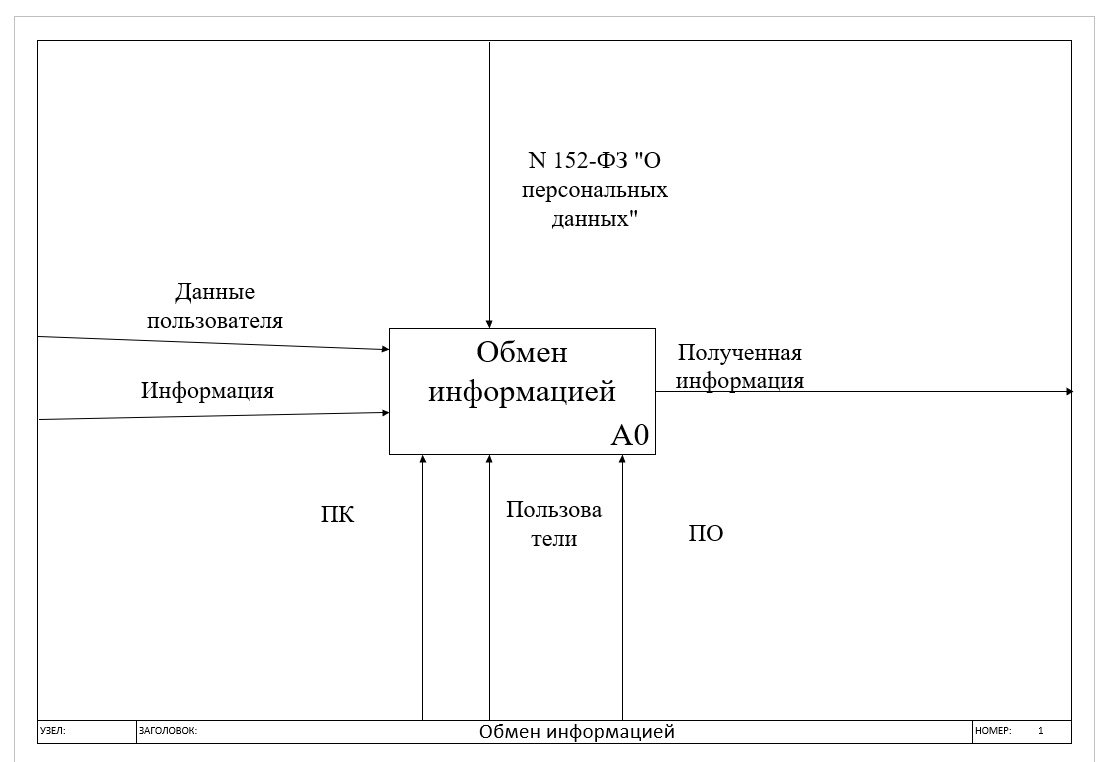
\includegraphics[width=0.5\textwidth]{assets/idef0.png}
      \caption{Диаграмма IDEF0}
    \end{figure}
  \end{center}
  
\end{frame}



\begin{frame}
  \frametitle{Онлайн форум SemiColon}
  
\begin{center}
    \huge{Информационная структура}
  \end{center}
  \begin{figure}
    \centering
    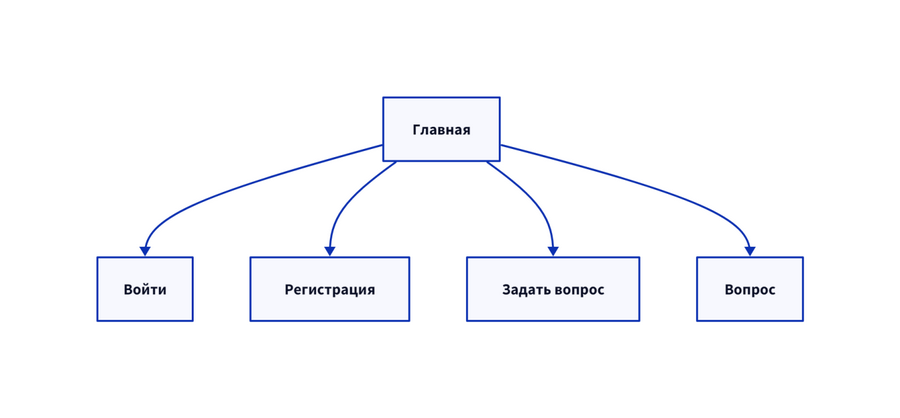
\includegraphics[width=0.9\textwidth]{assets/struct.png}
  \end{figure}
\end{frame}
\begin{frame}
  \begin{figure}
    \centering
    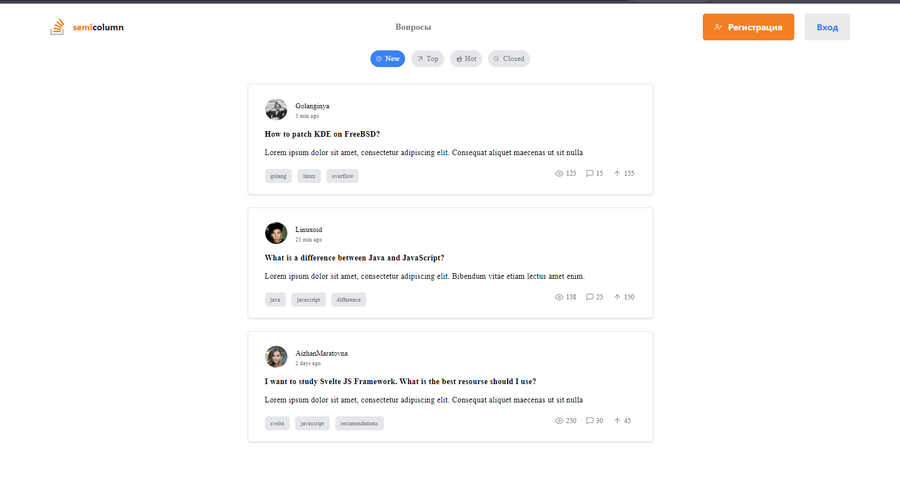
\includegraphics[width=1\textwidth]{assets/mainpage.png}
    \caption{Макет страницы "Главная"}
  \end{figure}
\end{frame}
\begin{frame}
  \begin{figure}
    \centering
    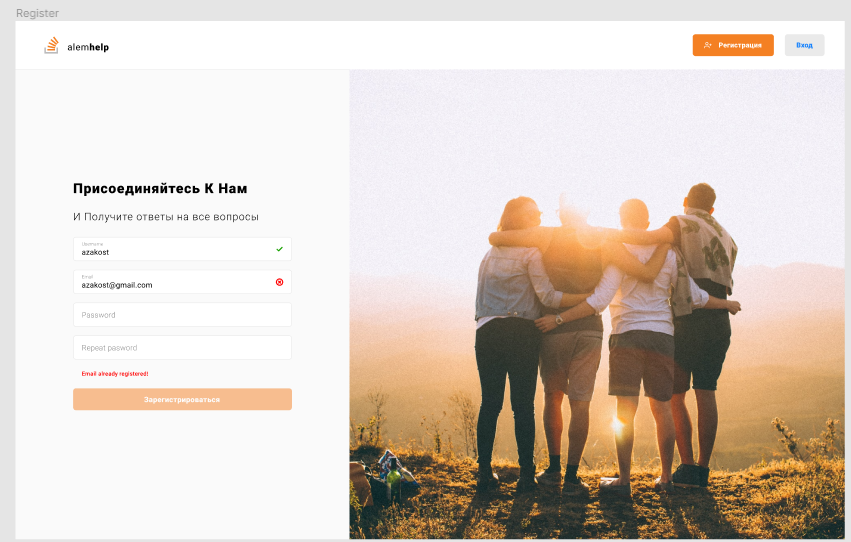
\includegraphics[width=1\textwidth]{assets/login.png}
    \caption{Макет страницы "Войти"}
  \end{figure}
\end{frame}
\begin{frame}
  \begin{figure}
    \centering
    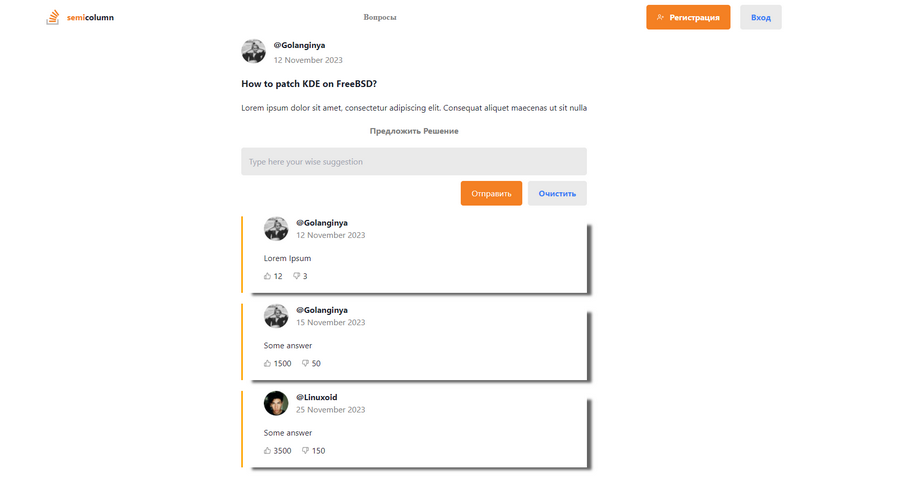
\includegraphics[width=1\textwidth]{assets/q.png}
    \caption{Макет страницы вопроса}
  \end{figure}
\end{frame}
\begin{frame}[fragile]
  \begin{minted}{html}
     <>
         <div className="header__auth">
            {typeof localUser === 'undefined' ? (
               <>
                  <button className="btn__register">
                     <img alt="user-plus" src={images.UserPlus} />
                     <Link to={'/auth/register'}>
                        <span>Регистрация</span>
                     </Link>
                  </button>
                  <Link to={'/auth/login'}>
                     <button className="btn__login">Вход</button>
                  </Link>
               </>
            ) 
  \end{minted}
\end{frame}
\begin{frame}[fragile]
  \begin{minted}{typescript}
  const addQuestion = (e: any) => {
    e.preventDefault()    
      let newQuestion: TQuestion = {
         id: uuid(),
         title: questionCreds.title,
         description: questionCreds.content,
         tags: questionCreds.category.split(', '),
         authorId: currentUser!.id,
         date: new Date().toLocaleString(),
         views: 0,
         comments: 0,
         upvotes: 0,
         answers: []
      }
      //@ts-ignore
      setQuestions([...questions, newQuestion])
      navigate('/')
   }

  \end{minted}
\end{frame}

\begin{frame}[fragile]
  \begin{minted}{typescript}
    const register = (e: any) => {
      e.preventDefault()
      let candidate = registeredUsers!.find(u => u.email == creds.email)
      if (candidate) {
         setLoginError(true)
      } else {
         let newUser: TUser = {
            id: uuid(),
            avatar: images.NoAvatar,
            email: creds.email,
            lastOnline: new Date().toLocaleString(),
            name: creds.name,
            password: creds.password,
            questionsIds: []
         }
         registerToStorage(newUser)!
         navigate('/')
      }
   }
  \end{minted}
\end{frame}

\begin{frame}
  \frametitle{Онлайн форум SemiColon}
    \begin{center}
    \huge{Заключение}
  \end{center}
  
  Была разработана клиентская часть веб-приложения онлайн форума, который поможет упростить и ускорить процесс обмена информацией
  В процессе создания веб-приложения был проведен анализ предметной области, выделены основные бизнес-процессы, созданы каркасы страниц, дизайн макеты страниц. Был реализован функционал для пользователя. Пользователь сайта может просматривать различные разделы сайта, просматривать и задавать вопросы, так же гость может зарегистрироваться и авторизоваться на сайте.

  \begin{center}
  \href{https://year3half2.vercel.app/}{\color{blue}{\underline{Демонстрация}}}  
  \end{center}
\end{frame}


\end{document}
